\section{Markov Decision Processes}
\label{sec:MDP}

Markov Decision Processes (MDPs) provide a straightforward means of modelling discrete-time optimization problems in which the actions of a single decision maker within an environment result in rewards and determine how the state of the environment changes in time. When there is a single decision maker we will refer to them as an agent. A typical example is an agent placed inside a maze; the agent takes actions to navigate the maze (forward, backward, left, right), and receives a constant reward of $-1$ after each decision. The environment terminates when the agent reaches the end of the maze. Given this reward signal, if an agent learns to maximize the sum of their rewards this is equivalent to saying that the agent has learned the quickest route to the end of the maze.

Formally, an MDP consists of a state space $\SS$ and an action spaces $\AA_s$ for each state $s \in \SS$. In situations where the action spaces are all the same we drop the subscript. The agent "enters" the environment according to an initial probability distribution $\mu_0$ over states. At each timestep $t$, the agent finds themselves in a state $s_t$ and must select and action $a_t \in \AA_{s_t}$. They transition to the next state $s_{t+1}$ according to a transition probability distribution $P_{s_ts_{t+1}}(a) = p(s_{t+1} | s_t, a_t)$ and also receive a reward according to a reward distribution $R(s_t, a_t) = p(r_t | s_t, a_t)$. A {\em finite} MDP is one in which the state space is finite, action spaces are finite, and the possible rewards received at each timestep are finite. An example of a finite MDP is shown below:

\begin{figure}
    \centering
    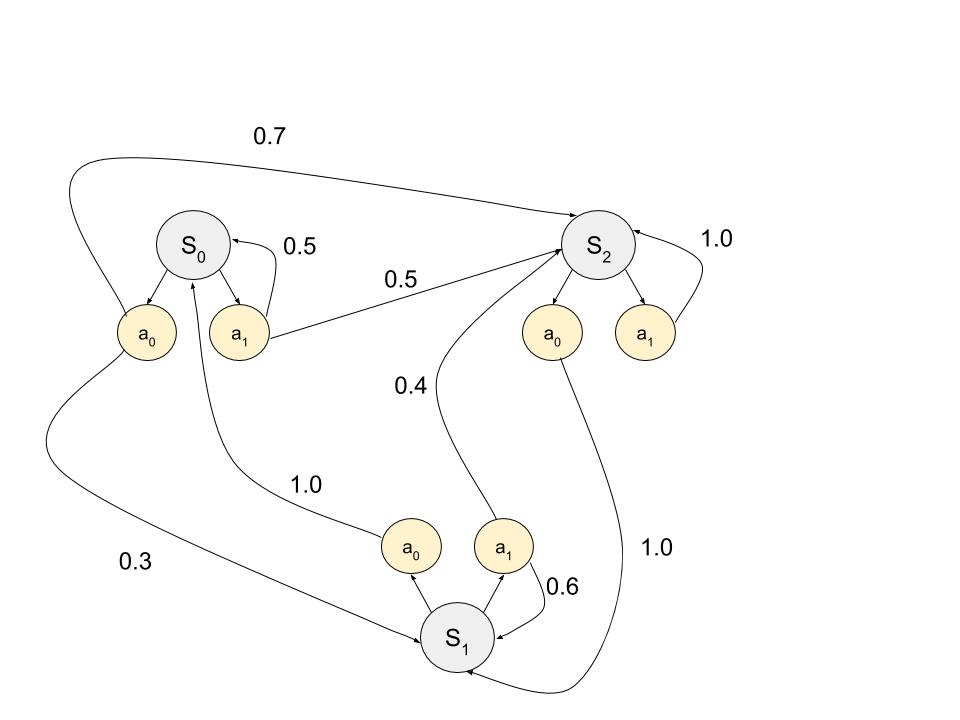
\includegraphics[scale=0.4]{images/simple_mdp.jpg}
    \caption{A finite MDP with 3 states and 2 actions in each state. The edges are labelled with the action-dependent probability transition.}
    \label{fig:simplemdp}
\end{figure}


Often, to deal with MDPs that last for arbitrary amounts of time, we introduce a {\em discount factor} $\gamma < 1$ that weights future rewards less than immediate rewards. This is to guarantee that infinite sums converge. 

In Chapters 2 and 3 we will specifically be dealing with {\em fixed-time episodic MDPs}. In such MDPs, the state of an agent is "reset" using $\mu_0$ every $T$ timesteps where $T$ is a fixed constant, and it is unnecessary to perform reward discounting, so we set $\gamma = 1$. When it is clear, we will drop $\gamma$ entirely from equations. Time plays as important role in the decision-making process of the agent in fixed-time episodic MDPs. Take for example a basketball player dribbling the ball up across halfcourt in the first quarter of a game. When there are 2 minutes left in the quarter, the player should continue to dribble the ball up and run a play with his teammates to maximize the chances of a scoring a field goal. Under essentially no circumstances should the player shoot the ball at halfcourt. In contrast, in the exact same situation, except with 2 seconds left in the quarter, the player should almost certainly shoot the ball. We should really consider these two different situations as separate states, even if everything else on the court is identical. We can view the state space of a fixed-time episodic MDP as branching at every timestep, and never returning to the same state or earlier states in a given episode. This structure is shown in Figure \ref{fig:finitemdp}.

\begin{figure}
    \centering
    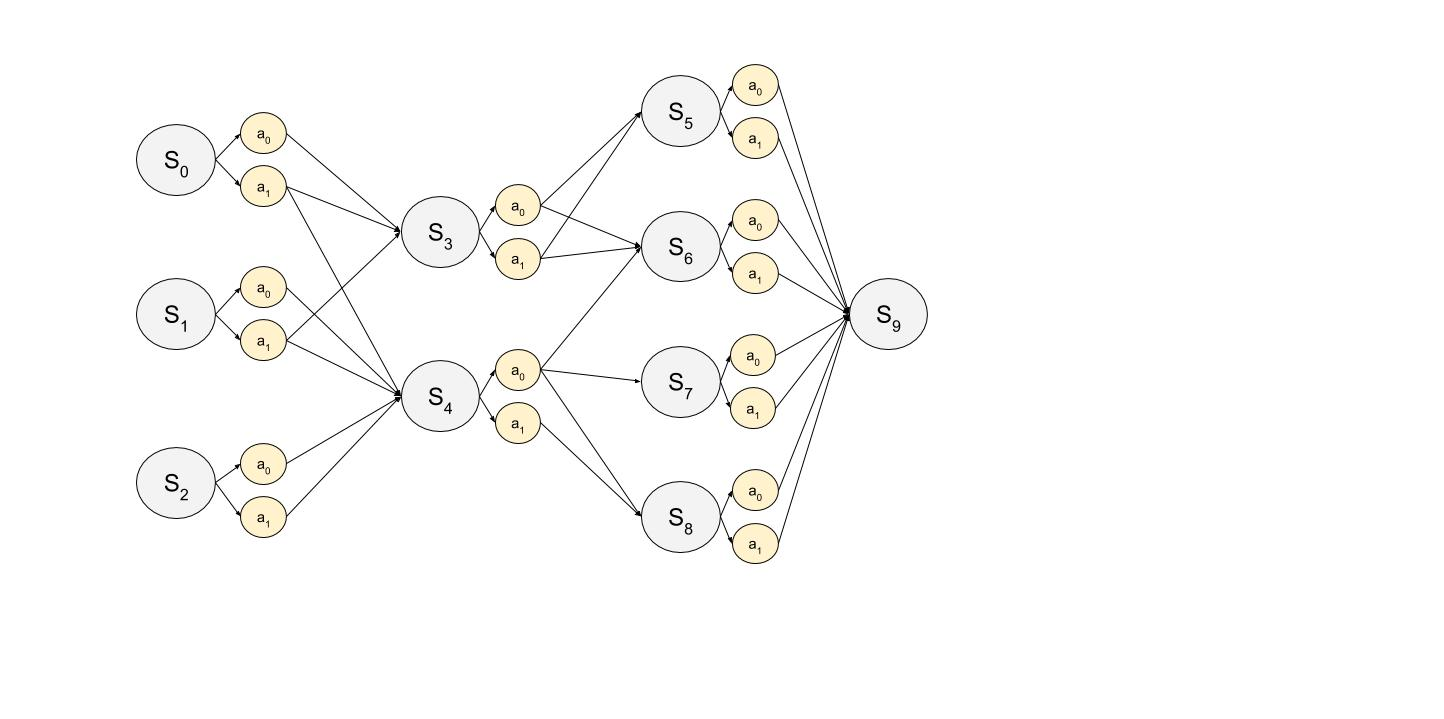
\includegraphics[scale=0.4]{images/fixed_time_finite_mdp.jpg}
    \caption{A finite 4 layer fixed-time MDP. There are 10 states, and two actions in every state except the final absorbing state. Transition probabilities are omitted to more clearly illustrate structure.}
    \label{fig:finitemdp}
\end{figure}

"Time" can become overloaded in this discussion, and so from now on we will refer to these $T$ timesteps as {\em layers}. A state being in layer $k$ means that it may only be encountered at the $k^{th}$ timestep in the MDP.

Next, we introduce some definitions that are important in discussing agent behavior in an MDP. 

\begin{mydef}
A {\em policy} $\pi$ is a complete specification for how an agent should select actions in each state. It consists of a collection of probability distributions $\pi_s$, indexed by state $s$, where each $\pi_s$ is a distribution over actions.
\label{mydef:policy}
\end{mydef}

\begin{mydef}
A policy $\pi$ is called deterministic if for each distribution $\pi_s$ there exists an action $a \in \AA_s$ such that $\pi_s(a) = 1$. 
\label{mydef:detpolicy}
\end{mydef}

\begin{mydef}
The {\em state value function} of a policy $\pi$ is the function
\begin{equation}
V_{\pi} : \SS \rightarrow \R
\label{mydef:vfinout}
\end{equation}

which maps a state to the expected sum of rewards that the agent will receive starting in state $s$ and behaving according to policy $\pi$. Explicitly it is given by the following equation:

\begin{equation}
V_{\pi}(s) = \mathbb{E}_{\pi}\left[\sum_{t=k}^T R_t(a_t,s_t) | s_k = s\right]
\label{eq:vfexpectation}
\end{equation}

\label{mydef:vf}
\end{mydef}


\begin{mydef}
A policy $\pi^*$ is called {\em optimal} or {\em a solution to the MDP} if

$$
\pi^* \in \text{argmax}_{\pi} \mathbb{E}_{s \sim \mu_0}\left[ V_{\pi}(s) \right]
$$
\end{mydef}

In other words, a policy $\pi^*$ is optimal if it maximizes the expected sum of rewards that an agent encounters during an episode. The following is a well-known fact about optimal policies in an MDP:

\begin{thm}
Every MDP admits a {\em deterministic} optimal policy $\pi^*$.
\label{thm:optimaldetpolicy}
\end{thm}

Chapter 4 adapts the well known Q-learning algorithm to a novel neural network architecture. To discuss Q-learning we must first introduce the action-value function.

\begin{mydef}
The {\em action-value} or {\em Q-value} function of a policy $\pi$ is the function which maps a state $s$ and state action $a \in \AA_s$ to the expected sum of rewards that the agent will receive starting in state $s$, taking action $a$, and then behaving according to policy $\pi$. Explicitly it is given by the following equation:

\begin{equation}
V_{\pi}(s, a) = \mathbb{E}_{\pi}\left[\sum_{t=k}^T R_t(a_t,s_t) | s_k = s, a_k = a \right]
\label{eq:qfexpectation}
\end{equation}

\label{mydef:qf}
\end{mydef}



There are two broad approaches to solving MDPs:
\begin{enumerate}
\item Model-based approaches such as dynamic programming
\item Model-free approaches, such as Q-learning and policy gradients
\end{enumerate}

These two approaches differ in their assumptions regarding agent sophistication. Model-based methods make the assumption that an agent has access to transition probabilities and reward functions, meaning they may use these quantities in calculating how to behave. They are so named because agents have "access to the model". In contrast, model-free methods do not make this assumption, and assume that agents only have knowledge of {\em their own experience}. Model-free methods are attractive as they represent a more realistic framework for "learning from scratch" as compared to model-based methods. The empirical study in Chapter 4 uses model-free methods, while our theoretical study of learning in stochastic games in Chapter 3 makes use of model-based approaches.


